
\section{实验验证}

本小节将对上文提出的算法作出实验验证,实验将分别构建基于树形拓扑的数据中心网络拓扑和基于随机生成的运营商网络拓扑,并在这些拓扑中验证本节的算法和通过带宽选择航点的算法之间的的差异性。

\subsection{实验环境}

本实验使用第二代编程独立于协议的数据包处理器行为模型作为软件交换机。使用基于IPv6的段路由作为段路由标准而不是基于标签预留协议的段路由,因为IPv6是未来IP网络的趋势。而且基于IPv6的段路由使用128位的SID,更具有可扩展性。本实验使用Linux命名空间来隔离网络堆栈,使用虚拟以太网(Virtual Ethernet, veth)来模拟交换机之间的接口。基于IPv6的段路由程序用P4语言开发,在BMv2上加载实现,控制器的功能则由一个python进程来实现,整体实验架构如下图所示。

\begin{figure}[htbp]
\setlength{\abovecaptionskip}{15pt plus 3pt minus 2pt}
\centerline{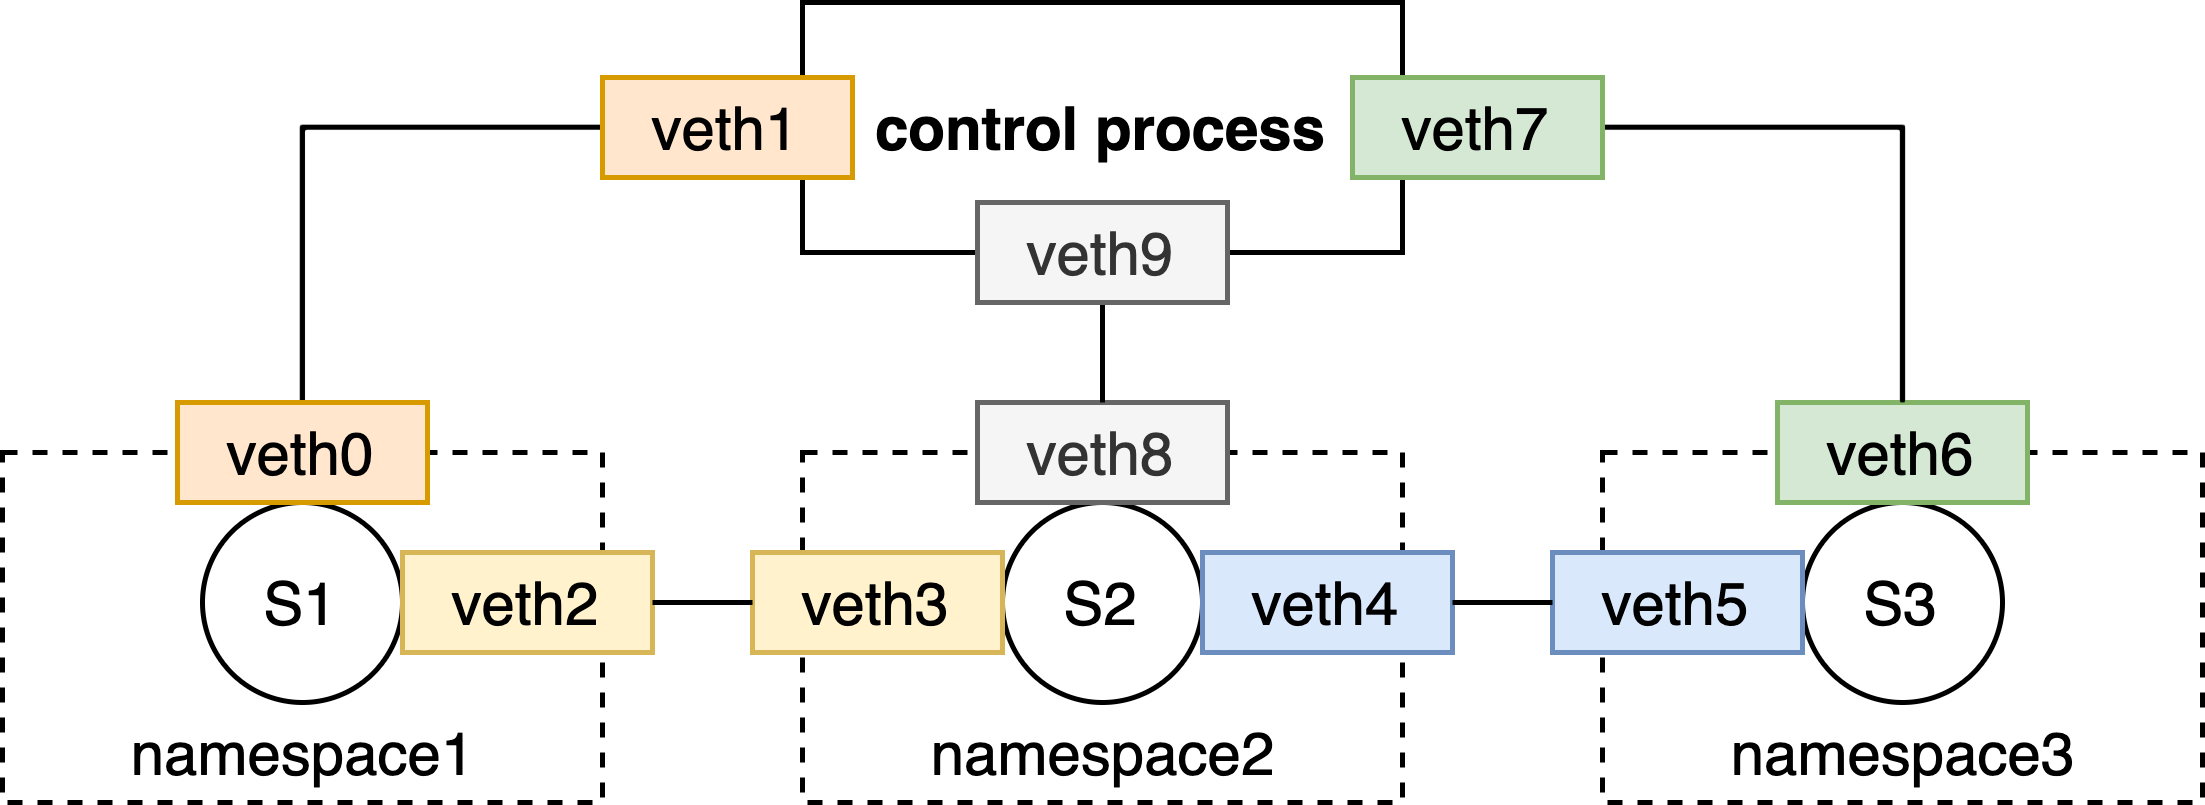
\includegraphics[width=0.8\textwidth]{./figures/ch3-test-env.png}}
\caption{实验环境示意图}
\label{fig-ch3-test-env}
\end{figure}

\subsection{实验步骤}

第一步启动网络拓扑,新建若干个网络命名空间,每一个网络命名空间相当于一个子网。将每对虚拟以太网绑定到对应的网络命名空间上并分配IPv4和IPv6地址。将设计好的拓扑中的每个虚拟交换机启动,加载编译的编程独立于协议的数据包处理器二进制文件,并的各个端口绑定到虚拟以太网上,这样在每对虚拟以太网间就形成连接两个虚拟交换机的链路。

第二步启动控制器,控制器将通过thrift接口和虚拟交换机BMv2建立带外通路进行控制流量传输。控制器将给所有虚拟交换机下发基础转发表项,包括二层广播表,等价多路径路由哈希组表,三层IPv6的路由器广告、邻居通告等代答表和三层IPv6路由表,使得全网拓扑中的节点可以用IPv6地址互通。

第三步在网络中选择两组相隔较远的节点,开始用流量生成软件Iperf持续性打流,保证在实验阶段网络处于有流量的动态状态。Iperf是一个用于网络性能测量和调优的工具。它是一种跨平台工具,可以为任何网络生成标准化的性能测量。Iperf具有客户端和服务器功能,并且可以创建数据流来测量两端之间的一个或两个方向的吞吐量。典型的 iperf 输出包含传输的数据量和测量的吞吐量的时间戳报告,本研究对时延结果数据的采集就是通过时间戳来获取。

第四步调整段路由航点选择算法参数,并启动段路由航点选择算法应用。

第五步选择一组源节点和目的节点开始从小流量开始打流,直到开始发生大规模的丢包,记录每次增加流量后控制器算法应用计算分配出的航点和端到端的时延情况。

第六步分析整理数据,得出结论。

\subsection{实验结果}

\begin{figure}[htbp]
\setlength{\abovecaptionskip}{15pt plus 3pt minus 2pt}
\centerline{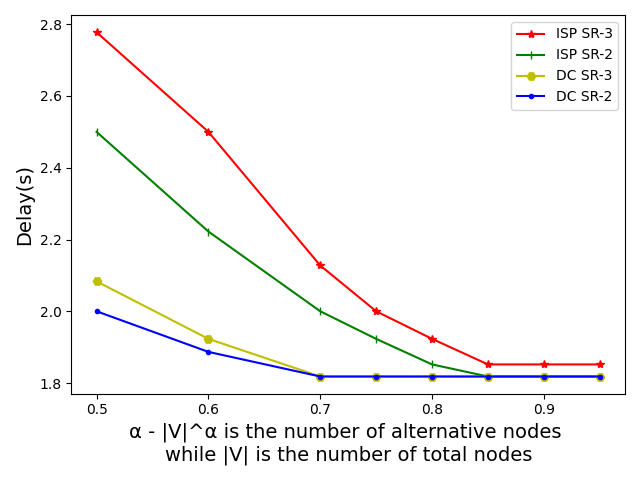
\includegraphics[width=0.8\textwidth]{./figures/ch3-test-1.png}}
\caption{$\alpha$取值测试结果图}
\label{fig-ch3-test-1}
\end{figure}

\begin{figure}[htbp]
\setlength{\abovecaptionskip}{15pt plus 3pt minus 2pt}
\centerline{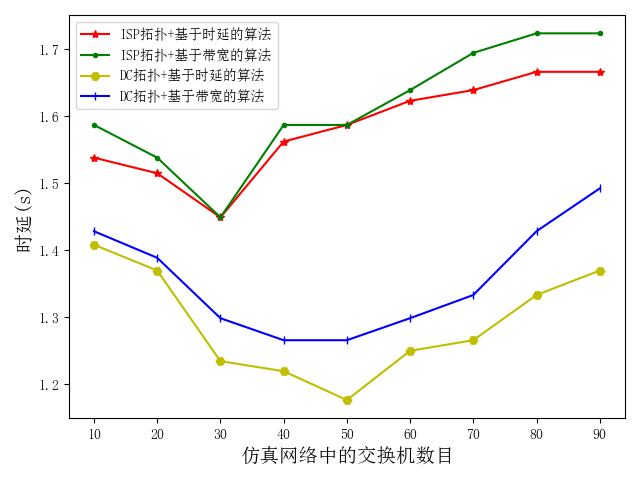
\includegraphics[width=0.8\textwidth]{./figures/ch3-test-2.png}}
\caption{平均延迟实验结果图}
\label{fig-ch3-test-2}
\end{figure}

\begin{figure}[htbp]
\setlength{\abovecaptionskip}{15pt plus 3pt minus 2pt}
\centerline{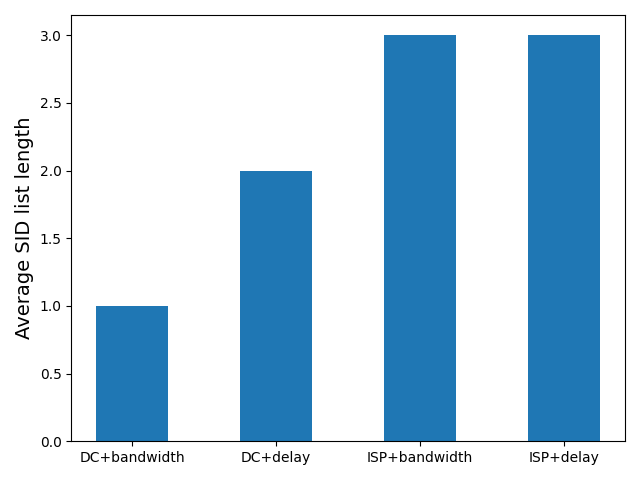
\includegraphics[width=0.8\textwidth]{./figures/ch3-test-3.png}}
\caption{标签列表长度实验结果图}
\label{fig-ch3-test-3}
\end{figure}

\begin{figure}[htbp]
\setlength{\abovecaptionskip}{15pt plus 3pt minus 2pt}
\centerline{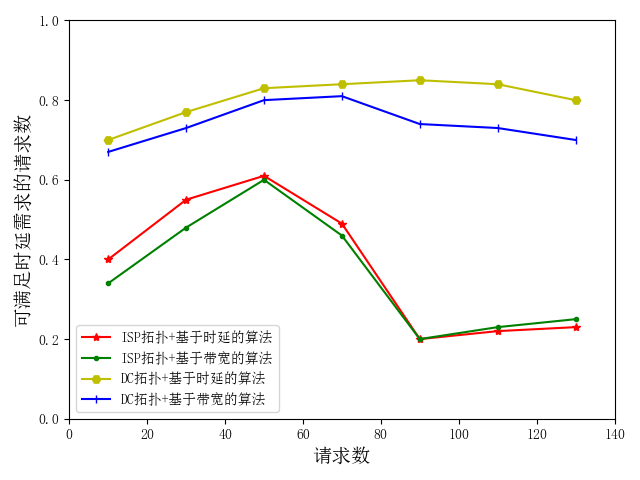
\includegraphics[width=0.8\textwidth]{./figures/ch3-test-4.png}}
\caption{保证请求延迟要求比例测试结果图}
\label{fig-ch3-test-4}
\end{figure}

1. $\alpha$取值测试

图3-a是为了验证候选节点占原拓扑全部节点的比率$\alpha$的取值。该试验将选择两个拓扑,一个是数据中心的树状拓扑结构,一个是随机生成的互联网服务提供商(ISP)拓扑。两个拓扑都具有40个节点;另外分别将段路由标签列表限制为2跳或3跳,即$SR-2$和$SR-3$。每一次确定参数$\alpha$的取值后后按照实验步骤3开始打流,记录iperf打流的时延结果。图中横轴是$\alpha$的大小,纵轴是延迟。

在数据中心的树状拓扑结构中,根据$SR-2$、$SR-3$进行比较,同时调整$\alpha$的值。可以看出,当选择$\alpha=0.7$时,在数据中心场景中SR-2和SR-3的情况下可以达到最佳值。其含义是:当节点集中有节点中心度在前${|V|}^{0.7}$的节点时。需要在计算中考虑时,已经可以得到效果最优的分段路由路径。而在互联网服务提供商拓扑中,使用随机拓扑进行模拟,在$SR-2$和$SR-3$的情况下,$\alpha=0.85$可以达到最优值。

2. 平均延迟实验

图3-b是为了验证在同样使用贝尔曼-福特算法作为标签列表选择核心算法的前提下,采用本文提出的链路权重以及生成辅助图的方案和直接用链路带宽作为权重的方案进行比较。实验的对照组同样是数据中心的树状拓扑结构和随机生成的互联网服务提供商拓扑。本实验的自变量是网络的大小,用网络拓扑中的交换机数目,即节点数目做为横坐标,因变量是打流的时延结果,并将其在纵坐标上描点,进而分析得出结论。如图3-b表明,当使用考虑时延的链路权重进行段路由标签列表计算时,无论使用树状拓扑结构还是随机拓扑结构,相对于直接使用带宽信息来计算来段列表,都能获得更低的平均延迟。

3. 标签列表长度实验

图3-c是为了验证3.3.1中提到的用段路由标签列表的长度被用来限制段列表生成算法,在数据中心的树状拓扑结构和互联网服务提供商随机拓扑结构中,分别使用了本文提出的基于带宽的贝尔曼-福特算法,以及本文提出的参考延迟的贝尔曼-福特算法。对四种场景下生成的段路由标签列表的平均列表长度进行比较。横坐标是四种测试场景,纵坐标是段标签列表的长度。本文提出的算法倾向于使用稍大的段列表长度,但考虑到贝尔曼-福特算法在生成段列表长度的时候会对长度进行限制,所以可以通过约束条件来保障段标签列表长度不会太长。本文使用的段标签列表都是2个或3个,因此可以认为没有产生额外的段列表标签开销。

4. 保证请求延迟要求比例测试

图3-d是为了验证使用本文提出的参考时延属性的段路由标签列表生成算法是否可以对时延需求进行保障。本实验的对比拓扑还是树状拓扑和互联网服务提供商拓扑,分别使用本文提出的参考延迟的贝尔曼-福特算法和基于带宽的贝尔曼-福特算法来计算给定服务请求数在10、50、90、130的情况下,可以分别保证请求延迟要求的比例。横坐标自变量是发起请求的数目,在实验中是从不同的源地址到目的地址进行打流,查看该流量被调度后的时延是否符合目标时延的需求,即实际时延小与目标时延,对满足时延需求的请求进行计数,与总请求数的比例就是纵坐标的数据。到可以看出,无论在树状拓扑结构还是互联网服务提供商拓扑中,本研究提出的算法都具有更好的延迟保证效果。

\section{算法结论}

在本章节中设计了一种参考链路时延构建链路权重选择段路由段列表的算法。该算法从多个角度测量并分析数据特性和研究的模型需求构成链路权重计算公式,通过对集中网络节点介数中心度进行分析得出用更少节点构建辅助图的拓扑降维方案,并使用贝尔曼-福特算法来推导计算出段列表。3.4的实验部分证明了该算法在时延保障上具有一定的有效性。

本文的算法仍有一些不足之处,例如,链路到达率是一个相当理想的值,在现实的网络中可能很难使用。此外,带内遥测的准确性会影响算法的结果,目前在商业交换机中,带内遥测数据是每3秒或10秒收集一次。因此,未来的工作是研究如何在算法中有效地收集和计算每个参数,并在物理网络中验证该算法。

\section{实验验证}

本章的实验是对分布式算法进行验证,因此除了对算法对时延效果的保障外,也会考虑算法的时间空间复杂度和时间复杂度。对比组主要有边界网关协议和开放最短路径优先的分布式协议,比较计算资源占用的情况、时延保障的效果和对网络吞吐量的影响,最终得出本章分布式段路由航点选择算法在时延保障上的有效性。本节将首先介绍实验设置,然后在数值和仿真实验中评估基于差分时延路径选择算法的性能和效果。

\subsection{实验环境}

1. 实验装置

本章提出的分布式段路由航点选择算法在实验验证中由C++实现。段路由节点主进程内有三个主要线程,第一个是用于对探测列表内段路由节点进行时延探测并更新时延矩阵的线程,第二个是接收其他段路由节点通告时延矩阵结论并更新时延矩阵的线程,第三个是对服务流量进行航点列表生成算法的进程。段路由节点的探测目标节点列表由控制器生成,通过管理配置的方式下发给段路由节点。

\begin{figure}[htbp]
\setlength{\abovecaptionskip}{15pt plus 3pt minus 2pt}
\centerline{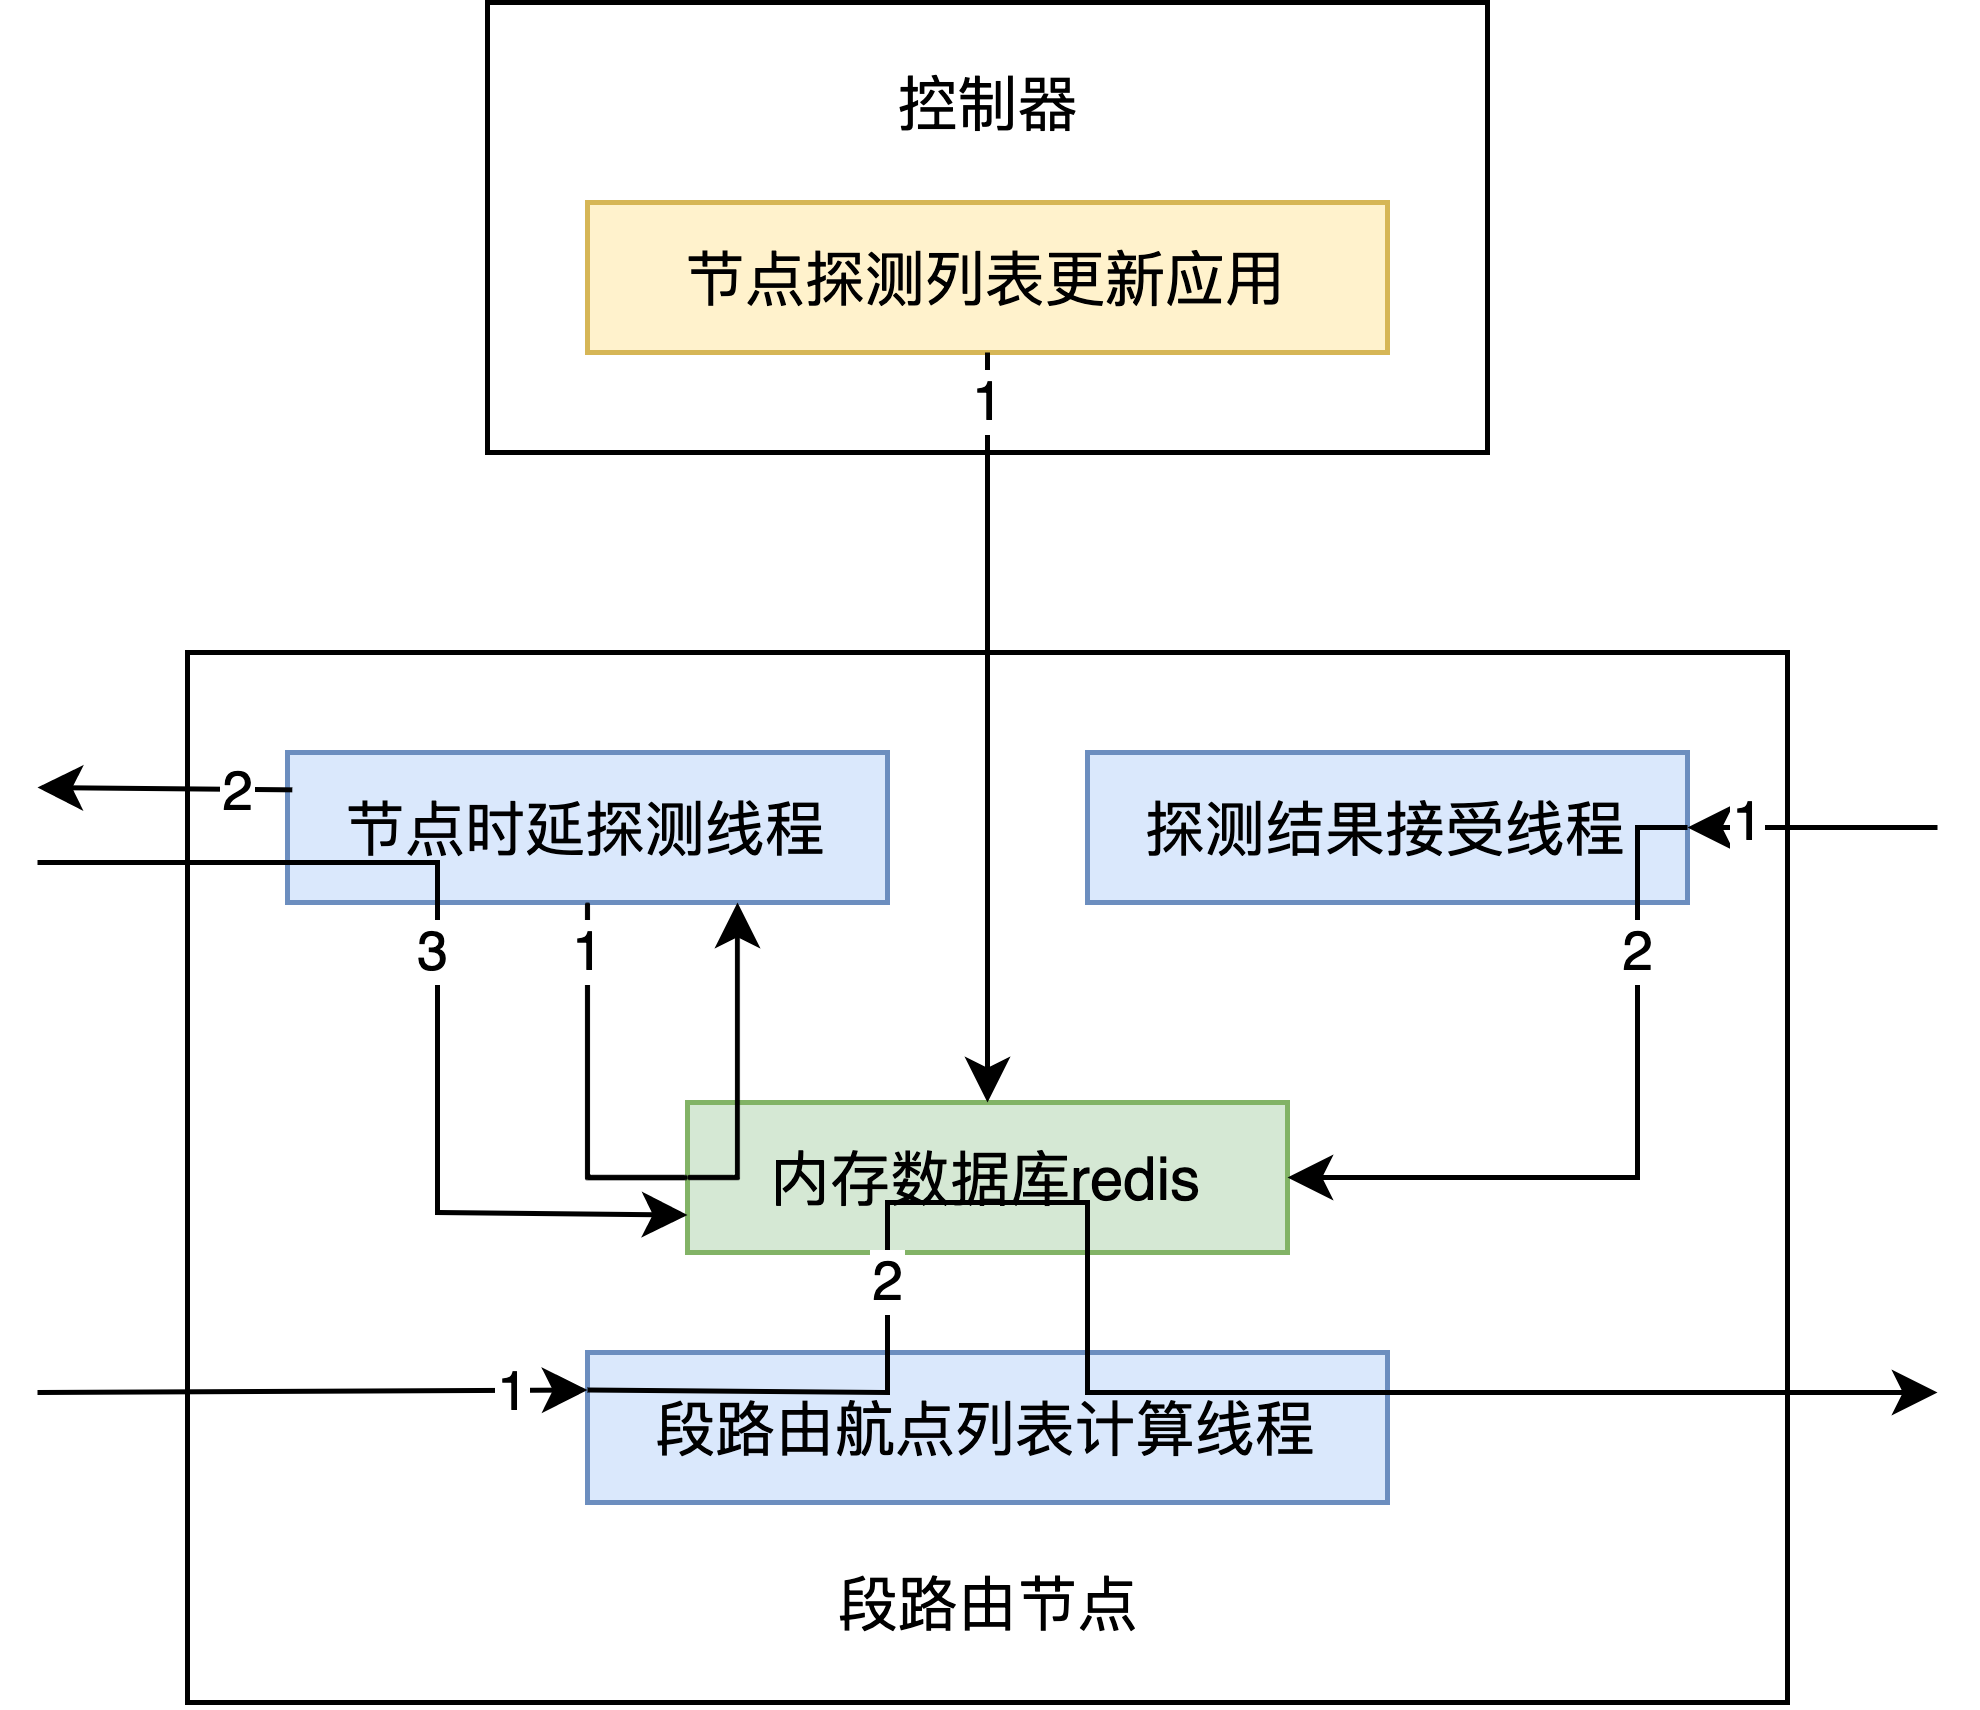
\includegraphics[width=0.8\textwidth]{./figures/ch4-test-code.png}}
\caption{实验代码结构示意图}
\label{fig-ch4-test-code}
\end{figure}
    
整个实验实现架构如图4-10所示:节点时延探测线程由计时器触发,第一步从内存数据库中获取需要进行时延探测的节点列表,第二步对外进行时延探测并记录结果,第三步将采集的结果与内存数据库中的差分时延矩阵数据进行比较并按照更新算法进行更新。探测结果接收线程由本节点的公告报文嗅探机制接收到其他段路由节点发送来的报文这一事件触发,第一步接收公告报文并处理报文内容,第二步将发布节点公告的时延的信息按照实验矩阵更新算法在内存数据库中进行更新。段路由航点列表计算线程由本节点的业务报文嗅探机制接收到带有目标时延请求的报文这一事件触发,第一步接受业务报文并提取目标地址和目标时延,第二步通过段路由航点列表生成算法生成段路由航点列表。

本文使用两种不同的段路由节点拓扑结构来评估基于差分时延的路径选择算法。数据中心拓扑由树状拓扑通过调惨生成,运营商网络通过随机网络生成,本文将通过调节拓扑的节点数来逐步验证本章提出的分布式段路由航点生成算法。

2. 实验流量

本章同第三章一样,仍然采用流量生成软件Iperf进行流量生成。主要发送TCP流量,这是为了获取报文中详细信息的时间戳,来对算法的时延保障效果进行比对。

3. 对比方案

本章算法实验的对比方案主要有自我对比和与其他路由算法进行对比,自我对比的对照组是是否选择对段路由航点列表长度进行限制以及限制的长度;其他路由算法主要是基于最短路径原理的开放最短路径优先协议和边界网关协议,实验主要利用开放最短路径优先对比本章提出算法的实际使用下端到端的总跳数,主要利用边界网关协议比较本章提出算法对时延需求的保障效果。

\subsection{实验步骤}

实验步骤分为单点算法资源消耗对比实验步骤和网络时延保障实验步骤。

第一步启动网络拓扑,新建容器,每一个容器相当于一个段路由节点,每个容器中运行模拟边界网关协议的自由范围路由进程或者运行本章提出的算法实现进程。将虚拟以太网的两端分别绑定到对应的容器分配的端口上并分配IPv6地址,启动开放最短路径优先应用生成基本路由表,这样在每对虚拟以太网间就形成连接两个虚拟交换机的链路。

第二步将设计好的拓扑中的每个段路由节点中的算法进程启动,控制应用将初始化内存数据库中每个节点的时延探测列表,段路由节点中的探测结果接收线程和段路由航点列表计算线程将开始监听各个绑定虚拟以太网的端口嗅探公告时延数据包和服务请求数据包。

第三步在网络中选择两组相隔较远的段路由节点容器,开始用流量生成软件Iperf持续性打流,保证网络运行在有基础流量的动态环境下。

第四步调整分布式段路由航点选择算法参数,例如选择限制段路由列表长度还是不限制段路由列表长度,调整惩罚值半衰期的时间等参数。

第五步选择一个源节点和目的节点开始从小流量开始打流,直到开始发生大规模的丢包,记录每次增加流量后两端航点端到端的时延情况。

第六步分析整理数据,得出结论。

\subsection{实验结果}

\begin{figure}[htbp]
\setlength{\abovecaptionskip}{15pt plus 3pt minus 2pt}
\centerline{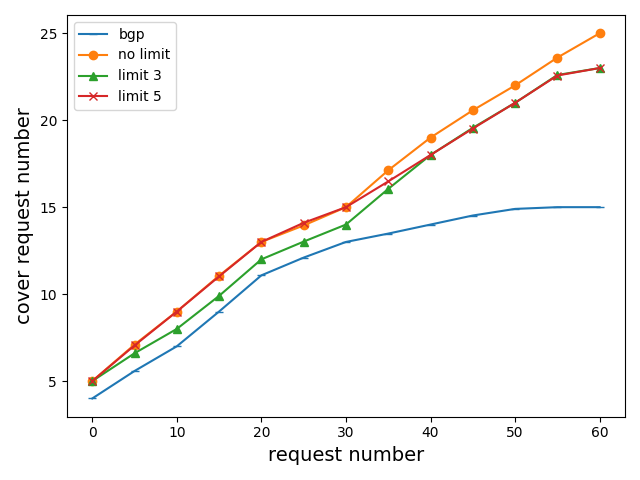
\includegraphics[width=0.8\textwidth]{./figures/ch4-test-tree-topo.png}}
\caption{树状拓扑下与边界网关协议对时延需求保障的比较结果图}
\label{fig-ch4-test-tree-topo}
\end{figure}

\begin{figure}[htbp]
\setlength{\abovecaptionskip}{15pt plus 3pt minus 2pt}
\centerline{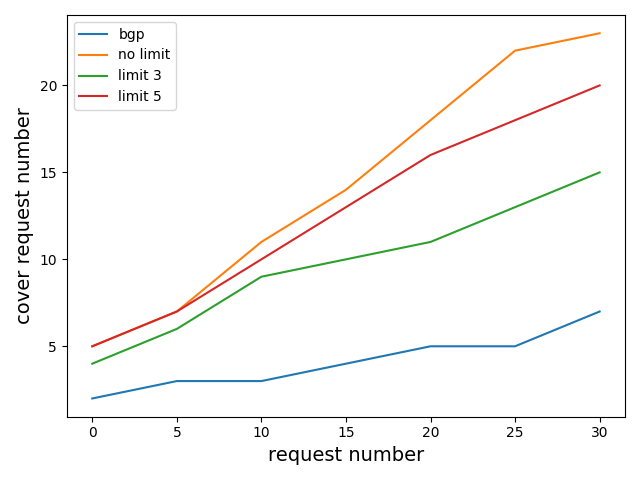
\includegraphics[width=0.8\textwidth]{./figures/ch4-test-random-topo.png}}
\caption{随机拓扑下与边界网关协议对时延需求保障的比较结果图}
\label{fig-ch4-test-random-topo}
\end{figure}

\begin{figure}[htbp]
\setlength{\abovecaptionskip}{15pt plus 3pt minus 2pt}
\centerline{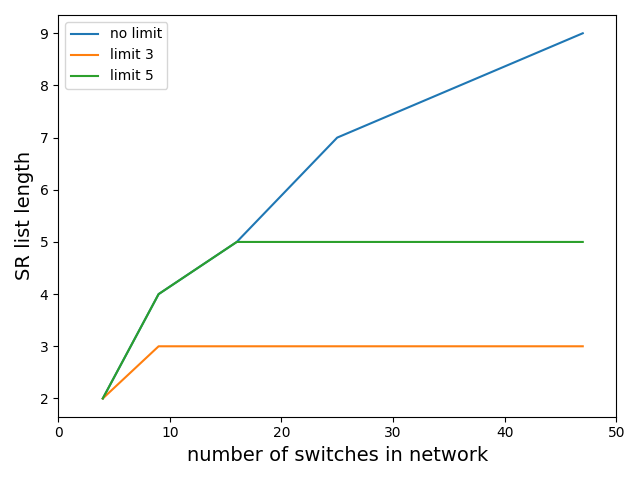
\includegraphics[width=0.8\textwidth]{./figures/ch4-sl-length.png}}
\caption{段路由标签列表长度分布结果图}
\label{fig-ch4-sl-length}
\end{figure}

\begin{figure}[htbp]
\setlength{\abovecaptionskip}{15pt plus 3pt minus 2pt}
\centerline{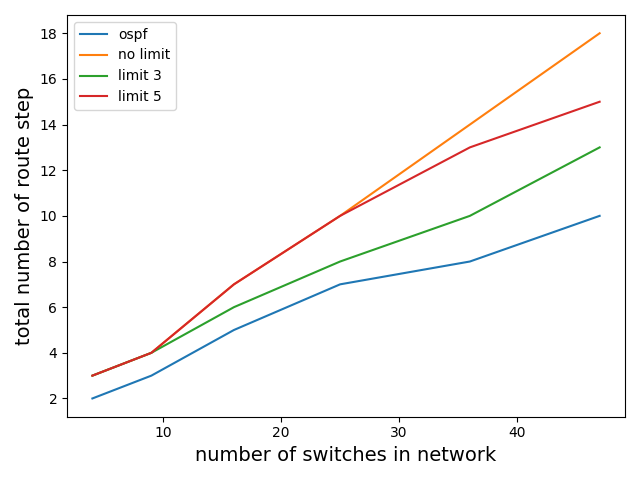
\includegraphics[width=0.8\textwidth]{./figures/ch4-total-length.png}}
\caption{基于差分时延的路径选择算法和最短路径算法的跳数对比结果图}
\label{fig-ch4-total-length}
\end{figure}
                
1. 树状拓扑下与边界网关协议对时延需求保障的比较

本实验是为了验证在同样使用数据中心树状拓扑的前提下,采用本章提出的保障时延的分布式段路由航点标签列表生成算法是否比边界网关协议有更好的时延需求保障能力。在第三章提到的算法中分析了段路由列表太长会带来的问题,并且建议不要使用过长的段路由列表,而在本章的算法中,具有对段路由标签长度进行限制和不进行限制的两种可选项,因此本实验将测试对段路由标签列表长度进行限制是否会大幅度影响路由调度的实验保障结果。本实验的自变量是服务请求的数目,这些服务请求到达时会携带一个期望的时延需求,因此用服务请求数目做为横坐标,因变量是可以满足时延需求的请求的数目,并将其在纵坐标上描点。本实验的对照组为运行边界网关协议和运行不限制标签列表长度的本章算法下,流量对时延结果的保障情况。分析实验结果数据可以初步得出结论:本章提出的分布式段路由航点标签列表生成算法确实比平常使用的分布式协议更能较好地保障业务的时延需求,段路由标签列表长度限制在3的时候,也可以达到较好的时延保障效果。

2. 随机拓扑下与边界网关协议对时延需求保障的比较

本实验与实验2类似,区别是将实验拓扑设置为模拟运营商网络的随机拓扑。本实验的自变量是在随机网络拓扑中携带目标时延发起服务请求的请求数目,并用该服务请求数目做为横坐标,纵坐标为可以满足其对应时延需求的服务请求的数目。本实验的对照组为运行边界网关协议和运行不限制标签列表长度的本章算法下,流量对时延结果的保障情况。通过分析实验结论数据可以得出结论,本章提出的分布式段路由航点标签列表生成算法在模拟运营商网络的随机网络拓扑中也能比其他路由协议更好地保障业务流量的时延需求,而段路由标签列表长度限制在5的时候,也可以达到和不限制下相当的较好的时延保障效果。

3. 基于差分时延的路径选择算法对段路由标签列表长度分布

当不对段路由标签列表长度进行限制的情况下,本章算法生成的段路由标签列表长度会因网络规模的扩大而增加,因此本实验主要是验证算法生成的段路由标签列表长度随着网络规模的扩大会呈现怎样的分布。本实验自变量时网络中段路由节点的数目,纵坐标因变量则是10个服务请求下计算出段路由航点列表的平均长度,对照组有对标签列表长度进行限制的算法结果段路由航点列表的平均长度。由实验结果可以看出,在不加限制的情况下段路由标签列表会和网络拓扑大小基本成线性增长,而限制段路由航点列表长度则会将标签列表长度固定,因此得出结论本算法需要根据具体网络拓扑情况,在生成段路由标签列表的时候对列表长度进行限制。

4. 基于差分时延的路径选择算法和最短路径算法的跳数对比

本实验目的是对比本章提出算法的流量路径跳数是否过高,因为跳数过多会对网络带来较大的额外带宽开销,本实验自变量是网络中总节点的数目,因变量是报文在本章段路由航点列表生成算法得到的段路由列表指导下平均总跳数,对照组时同样拓扑和同样流量服务需求下,按照开放最短路径优先协议进行流量转发最终经历的总跳数的平均值。由实验结果可以看出,在不加限制的情况下段路由标签列表指导下的路由跳数会和网络拓扑直径大小基本成线性增长,并且总跳数比开放最短路径优先协议多4.7\%到23.5\%,而开放最短路径优先协议下的总跳数总是基本和网络直径相当。

\section{算法结论}

本文提出了一种分布式的段路由航点列表生成算法,用于在网络节点较多的广域网络中用分布式的方式提供基于段路由的低延迟路径流量调度服务。由于本章主要采用分布式,因此缺少了软件定义网络下控制器集中式的网络优化途径,但也正因为没有使用集中式控制器使得本章提出的算法可以较为简单地在更大的网络内直接部署。本章算法的核心在于差分时延矩阵的生成、更新和选择,本章对算法进行了详细的解释,并留出了一些参数可以在实验或者真实场景部署阶段进行调整,例如惩罚值的压制阈值等。最后本章通过实验验证了该段路由航点列表生成算法生成的短路有策略是可以有效保障流量需求时延的。并且对数据中心拓扑和运营商拓扑分别适合的段路由标签列表长度进行了测试,最终本算法要求在使用时根据拓扑的情况配置段路由航点列表的长度限制,这是为了防止过长的段路由航点列表造成较低的链路有效负载和造成过多的端到端总跳数降低整个网络的吞吐量。

\chapter{段路由航点生成算法实验验证}

\section{引言}



\section{实验环境}

\section{基础实验}

\section{组网实验}

% \section{算法结论}

% 测试所有参考文献类型\cite{CITATION_BOOK,CITATION_ARTICLE,CITATION_PROCEEDINGS,CITATION_INPROCEEDINGS,CITATION_TECHREPORT,CITATION_STANDARD,CITATION_PATENT,CITATION_NEWSPAPER,CITATION_ELECTRONIC,SRSURVEYS}。

%% 本章参考文献
\ifx\usechapbib\empty
\nocite{BSTcontrol}
\setcounter{NAT@ctr}{0}
\bibliographystyle{buptgraduatethesis}
\bibliography{bare_thesis}
\fi
